\section{仮説の照合の詳細}\label{sup:inverse}
\begin{figure}[p]
  \centering
  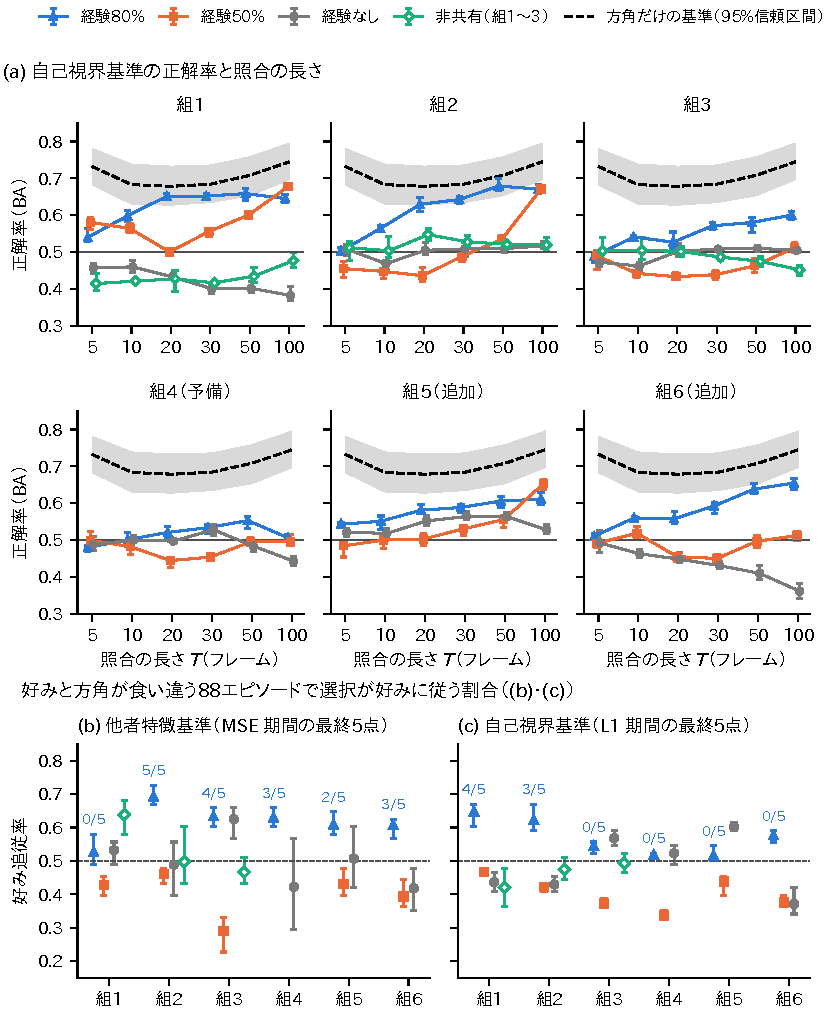
\includegraphics[width=\linewidth]{figs/inverse}
  % 図6：実験4。(a) BA と目標のフレーム数 T（自己視界基準）。経験80%・経験50%・経験なし・非共有条件を組ごとに。
  %   方角だけの基準の BA を同じ軸に描く。0.5 に横線。
  % (b) 食い違う 88 エピソードでの好み追従率（他者特徴基準は MSE 期間の最終5点，自己視界基準は L1 期間）。6組。
  % 元：data/result/v14/summary_figs/fig1_ba_vs_T.png・fig2_follow_pref.png
  \caption{仮説の照合．(a) 自己視界基準での好みの候補の選択の balanced accuracy と，誤差を足し合わせるフレーム数 $T$ の関係（組1〜6．方角だけの基準を並べる）．(b)(c) 好みと方角が食い違うエピソードで選択が好みに従う割合．(b) 他者特徴基準（MSE 期間の最終5点），(c) 自己視界基準（L1 期間の最終5点）．}
  \label{fig:inverse}
\end{figure}

\begin{table}[tbp]
  \centering
  \small
  \caption{仮説の照合の結果}
  \label{tab:inverse}
  % paper/tables/inverse.tex -- generated by analyze/paper/tables_paper.py; sources in paper/tables/README.md
\setlength{\tabcolsep}{3.5pt}%
\begin{tabular}{@{}lllll@{}}
\toprule
\multicolumn{5}{@{}p{0.9\linewidth}@{}}{(a) 自己視界基準の正解率 BA（$T=50$，L1 期間の最終5点の範囲，括弧は合格の点）} \\
\midrule
組 & 経験80\% & 経験50\% & 経験なし & \\
\midrule
組1 & 0.641〜0.671（5/5） & 0.598〜0.603（5/5） & 0.389〜0.420 & \\
組2 & 0.667〜0.701（5/5） & 0.526〜0.546（0/5） & 0.499〜0.518 & \\
組3 & 0.553〜0.593（4/5） & 0.445〜0.483（0/5） & 0.506〜0.517 & \\
組4 & 0.532〜0.564（2/5） & 0.486〜0.507（0/5） & 0.469〜0.494 & \\
組5 & 0.589〜0.618（0/5） & 0.534〜0.567（0/5） & 0.557〜0.574 & \\
組6 & 0.626〜0.653（5/5） & 0.479〜0.513（0/5） & 0.392〜0.432 & \\
\midrule
方角だけの基準 & \multicolumn{4}{l}{0.708 [0.653, 0.759]（素の一致率 0.707）} \\
 & \multicolumn{4}{l}{規則の一歩が少ない3分の1：0.614 [0.522, 0.704]（117エピソード，素の一致率 0.607）} \\
\midrule[\heavyrulewidth]
\multicolumn{5}{@{}p{0.9\linewidth}@{}}{(b) 経験80\%条件の他者特徴基準の合格の点，好み追従率（他者特徴基準は MSE 期間，自己視界基準は L1 期間の最終5点の範囲，括弧は CI の下限 $>0.5$ の点）} \\
\midrule
組 & 他者特徴基準 & 好み追従率 & 好み追従率 & \\
 & 合格の点 & 他者特徴基準 & 自己視界基準 & \\
\midrule
組1 & 5/5 & 0.489〜0.580（0/5，満たさなかった） & 0.602〜0.670（4/5） & \\
組2 & 5/5 & 0.670〜0.727（5/5，満たした） & 0.591〜0.670（3/5） & \\
組3 & 4/5 & 0.602〜0.659（4/5，満たした） & 0.523〜0.557（0/5） & \\
組4 & 5/5 & 0.602〜0.659（3/5，満たした） & 0.511〜0.523（0/5） & \\
組5 & 5/5 & 0.580〜0.648（2/5，満たさなかった） & 0.500〜0.545（0/5） & \\
組6 & 5/5 & 0.568〜0.625（3/5，満たした） & 0.557〜0.591（0/5） & \\
\midrule[\heavyrulewidth]
\multicolumn{5}{@{}p{0.9\linewidth}@{}}{(c) 経験80\% $-$ 非共有（自己視界基準の BA，$T=50$．組1〜3）：合格の点，ep200 の差 [95\%信頼区間]} \\
\midrule
組1 & \multicolumn{4}{l}{5/5，$+0.255$ [$+0.185$, $+0.324$]} \\
組2 & \multicolumn{4}{l}{5/5，$+0.157$ [$+0.088$, $+0.229$]} \\
組3 & \multicolumn{4}{l}{5/5，$+0.107$ [$+0.037$, $+0.177$]} \\
\bottomrule
\end{tabular}

  % 表5：組1〜6 の経験80%・経験50%・経験なしの BA（自己視界基準，T=50，最終5点の範囲）と合格の点，
  % 他者特徴基準の合格の点，好み追従率の点と書き方（好み／方角），経験80%−非共有（組1〜3），方角だけの基準の BA の行。
  % 出典：v14 まとめ §2 (1)〜(3)，v14_results_log §9。
\end{table}

\paragraph{正解率}
好みの候補を入れ比べて予測誤差の小さい方を選ぶと，経験80\%条件では偶然を上回って A-2 の好みを選べた（図\ref{fig:inverse}(a)，表\ref{tab:inverse}）．
自己視界基準の BA（$T=50$）は，経験80\%条件の本番の3組で $0.553$〜$0.701$ で，3組とも経験なし条件との差が合格の形になった（事前登録した主の判定に合格）．
経験50\%条件では，合格の形になったのは組1だけで（$0.598$〜$0.603$），主の判定は不合格であった．
全6組では，経験80\%条件で4組，経験50\%条件で1組が合格の形になった．
組4・組5 は単独では合格の形にならなかった．
組5では経験なし条件そのものの BA が $0.557$〜$0.574$ と 0.5 を上回り，経験80\%条件との差（$+0.015$ [$-0.040$, $+0.075$]）が出なかった．
また，組1・組6 の差の一部は，経験なし条件の BA が 0.5 を下回ったこと（組1 $0.389$〜$0.420$，組6 $0.392$〜$0.432$）による．
他者側の特徴予測の誤差で選んだ場合（他者特徴基準）も，経験80\%条件の本番の3組で合格の形になった（BA $0.73$〜$0.79$）．
% 出典：v14 まとめ §2 (1) 表，v14 ログ §27 A・B・§43・§44，執筆メモ §5 主張5。

非共有条件では照合は成り立たなかった．
非共有条件の BA は $0.42$〜$0.53$ で，同じ組・同じエピソードの経験80\%条件は3組とも5点すべてで上回った．
非共有条件の選択は，好み×配置に沿って入れ替わらず，一方の候補に偏っていた．
これも構成から予想された確認である．
% 出典：v14 まとめ §2 (3)，v14 ログ §40。

\paragraph{方角で説明できるか}
A-2 の好みは，A-2 がその間に進んだ方角とも結びついている．
A-2 の $t=1$〜50 の変位の向きだけで候補を選ぶと，好みの正解と 0.707 の割合で一致し，BA は 0.708 [0.653, 0.759] であった（方角だけの基準．規則の一歩が少ない3分の1では 0.614 [0.522, 0.704]）．
これは経験80\%条件のモデルの BA（0.53〜0.70）と同じかそれより高い．
したがって，正解率が偶然を上回ったことだけから，モデルが方角以上の手がかりを使ったとは言えない．
なお，方角だけの基準は A-2 の本当の位置を使うのに対し，モデルが使うのは A-1 の視界だけである．
% 出典：v14 ログ §18・§19（0.707），執筆メモ §5 主張5 の注意。BA は第1弾の指示書 §2.1 の 3 で Claude Code が出す。

そこで，好みの正解と方角の正解が食い違う 88 エピソードで，選択が好みに従う割合を調べた（図\ref{fig:inverse}(b)(c)）．
事前登録した条件（他者特徴基準，MSE 期間の最終5点）では，経験80\%条件の本番の3組のうち組2・組3 が好み追従基準を満たし，組1 は満たさなかった．
全6組では，組2・組3・組4・組6 の4組が満たし，組1・組5 は満たさなかった．
自己視界基準（主の判定と同じく L1 期間の最終5点で数えた記述）で同じ割合を見ると，好みに従ったのは6組中2組（組1・組2）であった．
二つの基準のどちらでも好みに従ったのは組2だけである．
経験50\%条件では，どちらの基準でも好みに従う組はなかった（他者特徴基準では，保存された出力のない組4 を除く）．
% 出典：v14 ログ §27 C・§21 B・§21 C，paper/check/follow_pref_late5.json（Claude Code 第1弾）。
% 数え方：v14 まとめ §5 の 3 の「L1 で s0・s1・s5，両方で s1・s5」は，s5 を MSE 期間のチェックポイントで数えたもの。
%   v14 ログ §21 B（MSE 期間の自己の視界の L1 は判定に使わない）に合わせ，L1 期間の最終5点で数え直した（2026-10-26 決定）。

この結果には三つの注意が要る．
第一に，経験なし条件の組3も同じ条件を満たした．
条件を満たすことだけでは経験の効果とは言えない．
第二に，A-2 が規則で動いた一歩が少ない3分の1のエピソードでは，どの組も条件を満たさなかった．
第三に，方角の条件は，経験50\%条件の結果を見た後に作ったものである（経験80\%条件の結果を見る前に登録した）．
方角だけの基準との差（モデルの BA $-$ 基準の BA，同じエピソードで対にしたブートストラップ）を事前登録外の確認として求めた．
主の自己視界基準では，経験80\%条件の差は6組とも負で，組をまたいだ差は $-0.089$ [$-0.140$, $-0.038$] であり，基準を上回った点はどの組にもなかった．
副の他者特徴基準では，経験80\%条件の差は6組とも正で，組をまたいだ差は $+0.049$ [$+0.026$, $+0.072$] と0を含まなかったが，組ごとに信頼区間の下限が0を上回ったのは組4（5点中5点）と組2（5点中2点）だけであった．
同じ他者特徴基準でも，経験50\%条件（$-0.044$ [$-0.087$, $-0.001$]，組4 を除く5組），経験なし条件（$-0.248$ [$-0.357$, $-0.138$]），非共有条件（$-0.260$ [$-0.361$, $-0.159$]，組1〜3）は基準を下回った．
% 出典：paper/check/direction_vs_model.json，paper_round2_log.md §5（Claude Code，測り方 d214f7d，結果 1de3742）。
なお，方角だけの基準は A-2 の本当の位置を使うのに対し，モデルが使うのは A-1 の視界だけである．

以上より，研究者が用意した二つの候補の判別は経験80\%条件で偶然を上回るが，主の自己視界基準での正解率は方角だけの基準を上回らず，副の他者特徴基準でも組をまたいでわずかに上回るにとどまった．好みと方角が食い違うエピソードについては，一部のモデルで方角に反して好みの側を選ぶ傾向が見られたが，好みに固有の情報による判別は確証されなかった．
方角だけの基準は最終的な変位の向きだけを見るので，位置の履歴や局所的な動きなど，ほかの単純な手がかりを使っている可能性も除けていない．
この結果は，限られた条件での候補の判別として読むべきであり，好みと方角を独立させた課題での確認が要る（本文5.5節）．
% 出典：v14 まとめ §5 の 1・2，v14 ログ §21・§27 C。

\paragraph{当てて選ぶか，書き出すか}
同じ経験80\%条件の段階Iのモデルで，候補を入れ比べて選ぶ場合（照合）と，1ビットモジュールに書き出させる場合（他者用モジュール）を比べた（図\ref{fig:write-choose}）．
1ビットモジュールを学習した組1〜3 の最終5点で，食い違うエピソードで好みに従う割合は，当てて選ぶと自己視界基準で 0.52〜0.67，他者特徴基準で 0.49〜0.73 と，多くの組で 0.5 を上回った．
書き出させると 0.30〜0.41 で，3組とも 0.5 を下回り，方角の側に寄った．
自分の経験から作られた見込みは，好みの候補ごとに異なる予測を生み，それを観察と照らすと好みをある程度区別できる．
しかし，他者用モジュールに学習させると，モジュールは同じ見込みを使って好みを書くのではなく，予測に役立つ方角や位置を書いた．
% 出典：当てて選ぶ＝Claude Code 第1弾の追加（paper_round1_log.md §7。自己視界基準は L1 期間，他者特徴基準は MSE 期間の最終5点。
%   組1 0.602〜0.670／0.489〜0.580，組2 0.591〜0.670／0.670〜0.727，組3 0.523〜0.557／0.602〜0.659），
%   書き出す＝v14 ログ §39（1ビット 0.30〜0.41，最終5点）。
%   v14 まとめ §2 (4) の 0.55〜0.66・0.57〜0.67 は組1〜3 の L1 期間 ep200 の1点で，数え方が違うので使わない。

\begin{figure}[tbp]
  \centering
  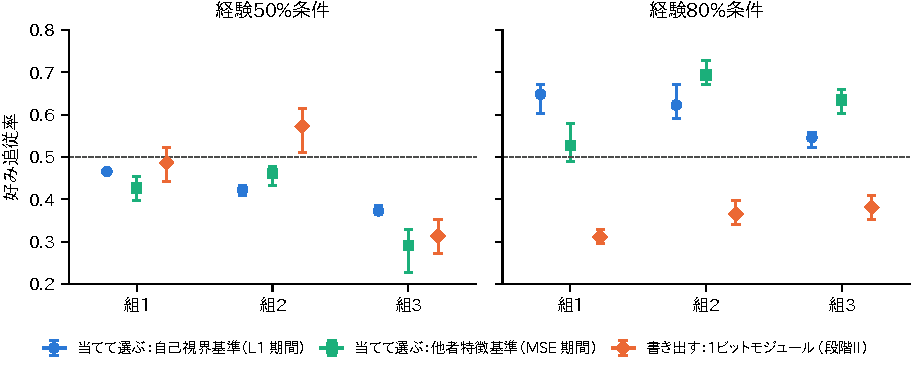
\includegraphics[width=0.8\linewidth]{figs/write_vs_choose}
  % 図5：好みと方角が食い違う 88 エピソードで，選択（または u）が好みに従う割合。
  % 「当てて選ぶ（照合）」と「書き出す（1ビットモジュール，実験3）」を，経験50%・経験80% で，組ごとに並べる。0.5 に横線。
  % 元：data/result/v14/summary_figs/fig3_write_vs_choose.png
  \caption{同じモデルで，候補を入れ比べて選ぶ場合と，他者用モジュールに書き出させる場合の比較．好みと方角が食い違うエピソードで好みに従う割合を，(a) 経験50\%条件と (b) 経験80\%条件で組ごとに示す．塗りの菱形は事前登録した1ビットモジュールの値，白抜きの菱形は事前登録外の値．破線は 0.5．}
  \label{fig:write-choose}
\end{figure}
